\paragraph{QuizziPedia::Front-End::Directives::UserDetailsDirective}

\label{QuizziPedia::Front-End::Directives::UserDetailsDirective}

\begin{figure}[h]
	\centering
	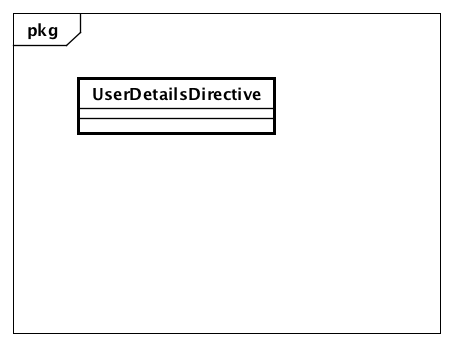
\includegraphics[scale=0.80,keepaspectratio]{UML/Classi/Front-End/QuizziPedia_Front-end_Directives_UserDetailsDirective.png}
	\caption{QuizziPedia::Front-End::Directives::UserDetailsDirective}
\end{figure}

\begin{itemize}
	\item \textbf{Descrizione}: directive che permette di visualizzare i dati personali di un utente;
	\item \textbf{Utilizzo}: permette di visualizzare i dati personali di un utente, in dettaglio conterrà:
	\begin{itemize}
		\item Username;
		\item Immagine.
	\end{itemize}
	\item \textbf{Relazioni con altre classi}:
	\begin{itemize}
		\item \textbf{OUT \texttt{UserView}}: view contenente i dati personali dell'utente, le sue statistiche relative ai questionari e agli allenamenti effettuati e i questionari a cui è iscritto;
		\item \textbf{OUT \texttt{OtherUserView}}: view contenente i dati personali e le statistiche di un utente ricercato;
		\item \textbf{IN \texttt{UserDetailsController}}: questa classe permette di gestire i dati di un utente da mostrare nella pagina di un profilo;
		\item \textbf{IN \texttt{UserDetailsModelView}}: classe di tipo modelview la cui istanziazione è contenuta all'interno della variabile di ambiente \$scope di \textit{Angular\ped{G}}. All'interno di essa sono presenti le variabili e i metodi necessari per il \textit{Two-Way Data-Binding\ped{G}} tra la directive \texttt{UserDetailsDirective} e il \textit{controller\ped{G}} \texttt{UserDetailsController}.
	\end{itemize}
	\item \textbf{Attributi}:
	\begin{itemize}
		\item \texttt{+ userDetails: Object} \\ Oggetto contenente i seguenti campi dati:
		\begin{itemize}
			\item \texttt{username: String} \\
			inserire descrizione campo qui
		\end{itemize}
		\item \texttt{+ controller: String} \\ Stringa contenente il nome del \textit{controller\ped{G}} della direttiva;
		\item \texttt{+ restrict: String} \\ Stringa che permette di definire le modalità di inserimento della direttiva all'interno della pagina;
		\item \texttt{+ scope: Scope} \\ Oggetto scope interno della direttiva, contiene le funzionalità per gestire i dati presenti all'interno;
		\item \texttt{+ templateUrl: String} \\ Stringa contenente il percorso del file \textit{HTML\ped{G}} che contiene la direttive.
	\end{itemize}
\end{itemize}